
\begin{figure}[b!]
\begin{center}
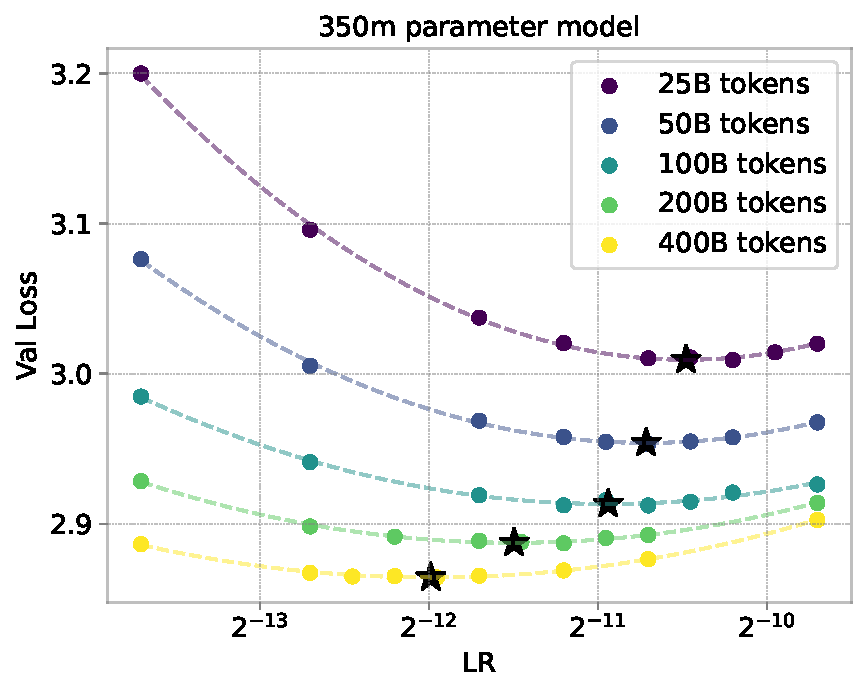
\includegraphics[width=0.7\textwidth]{images/350m.pdf}
\caption{Final validation loss as a function of learning rate (LR) and token horizon. The dashed lines indicate our fitted curve and the stars indicate optimal LR. The optimal LR decreases monotonically with longer horizons.}
\label{fig:350m_curves}
\centering
\end{center}
\end{figure}

\vspace{-0.3cm}

\section{Experiments}\label{sec:exps}


\textbf{Experimental Setup.} Our experimental setup closely follows the setup of the GPT-3 paper \citep{brown2020language}. We consider model sizes of 50 million (m), 125m, 350m, 760m, 1.3 billion (B), and 2.7B parameters using the architectures of Table 2.1 in the GPT-3 paper. The table is replicated as \Cref{table:param} in \Cref{appendix:hps} and also lists the LRs used in the GPT-3 paper. We use hyperparameters following GPT-3 -- weight decay of 0.1, gradient clipping of 1.0, and cosine learning decay schedule. The full list of hyperparameters can be viewed in \Cref{table:hps_appendix} in \Cref{appendix:hps}. The LR will vary with the training step since we use an LR schedule, and we will use the term LR to refer to the largest LR of a run. We make three adjustments compared to the GPT-3, mainly to prevent divergence of the model for high LRs. 1) For warmup we use the maxima of 1\% of the training steps following \cite{muennighoff2024scaling} and 1000. Having too short a warmup stage is known to cause divergence \citep{wortsman2023small} which we want to avoid for short training runs. 2) We use qk-norm following \cite{dehghani2023scaling}, this is known to prevent divergence without hurting validation loss \citep{wortsman2023small}. 3) The original GPT-3 paper uses different batch sizes for different model sizes. To avoid confounders we simply use the same batch size of 0.5m tokens all model. We use the RefinedWeb dataset \citep{refinedweb}, a common-crawl derived dataset of roughly 600B tokens which is known to be of high quality \citep{fineweb}. Experiments are run on the Megatron codebase \citep{shoeybi2019megatron}. Unless mentioned we will use the same seed for all runs. For curve fitting we use least-square fitting with either a first or second-degree polynomial using Numpy and Scipy \citep{numpy}, \rebuttal{and we always have more data points than free parameters in the fits.}



















\begin{figure}[]
    \centering
    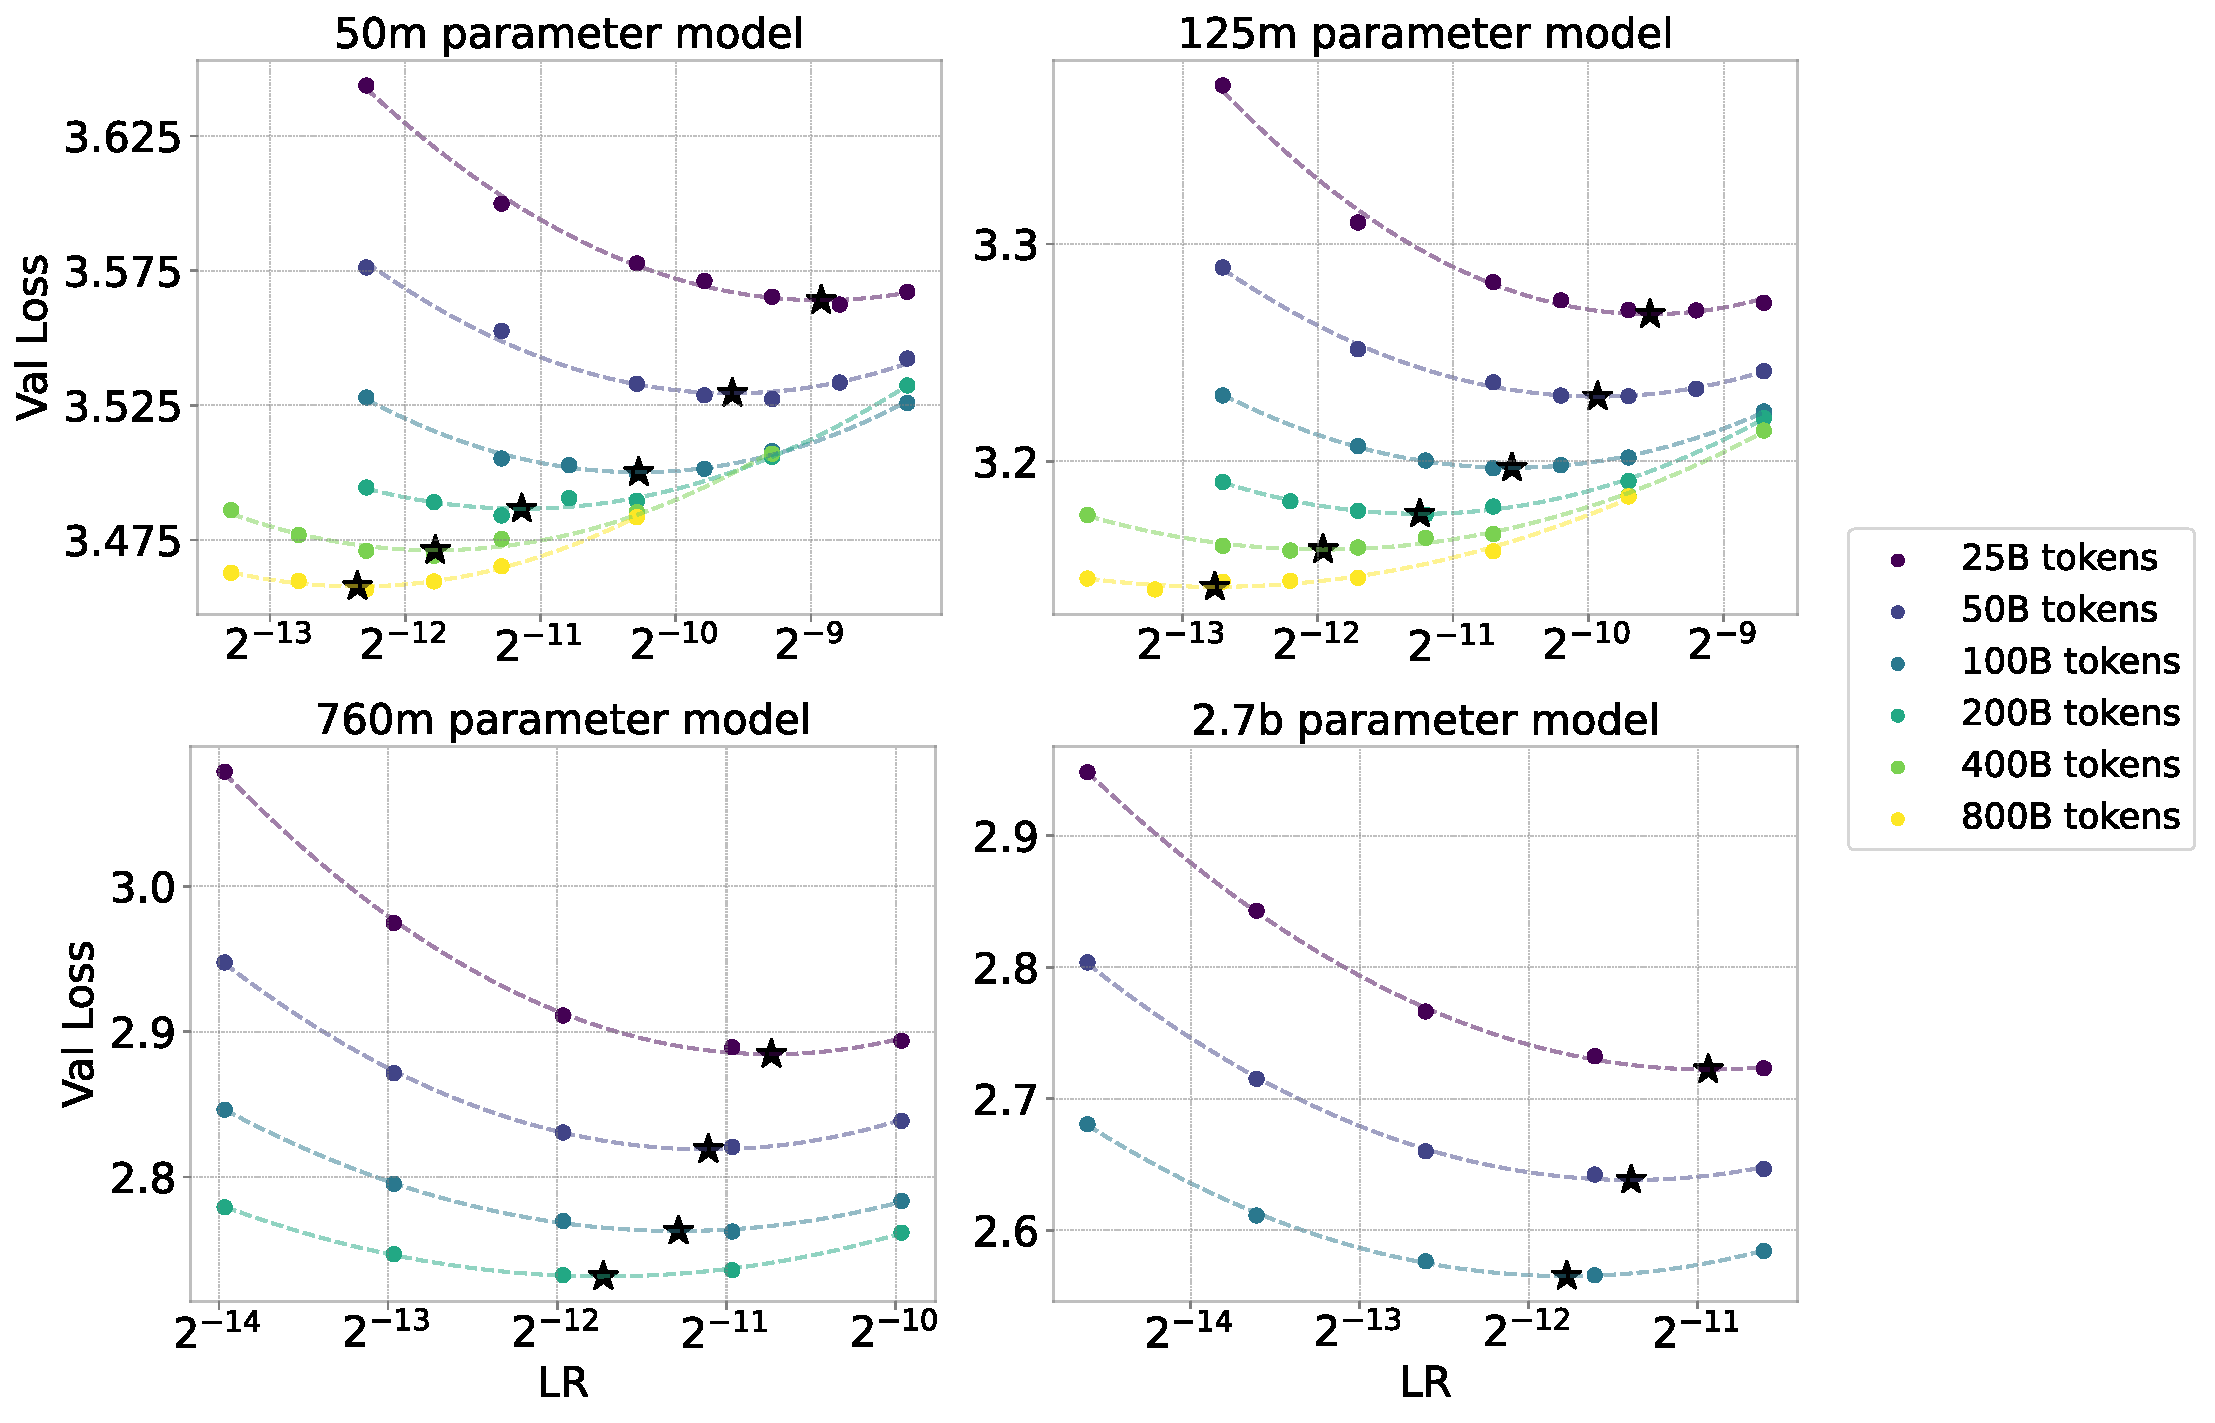
\includegraphics[width=\linewidth]{images/omnigraffle/legend_fix.pdf}
    \vspace{-0.3cm}
    \caption{Final validation loss as a function of max learning rate (LR) and token horizon for four models. The dashed lines indicate our fitted curve. The optimal LR, denoted by a black star, decreases monotonically with longer horizons for all models.}
    \label{fig:4curves}
    \vspace{-0.3cm}
\end{figure}


\subsection{Ablations}
\label{sec:initial_abl}






In our first experiment, we consider the 350m LLM model from \Cref{table:param} in \Cref{appendix:hps}. We perform an ablation study where we vary the LR and token horizon and measure the final validation loss. We consider  $\{25, 50, 100, 200, 400\}$ billion tokens. We will start with the LR of \scinot{3}{-4} from \Cref{table:param} which is what the GPT-3 paper used \citep{brown2020language}. We then multiply this base LR by factors $\{0.25, 0.5, 1, 2, 4\}$. The LRs we consider are thus $\{ \scinotmath{7.5}{-5}, \scinotmath{1.5}{-4}, \scinotmath{3}{-4}, \scinotmath{6}{-4}, \scinotmath{1.2}{-3} \}$. For each combination of LR and token horizon, we train a model and record its final validation loss. To make sure we have the best possible resolution around the minima we find the optimal learning rate $LR^*$, and then further train with the LRs halfway between $LR^*$ and its two nearest neighbors -- a procedure we repeat twice. From these losses, we fit a curve that estimates how the final validation loss depends on the LR. For each token horizon we fit a second-degree polynomial in $\log(LR)$, \rebuttal{using a quadratic polynomial as it provides an excellent fit and is the simplest polynomial with a well-defined minimum.} The $R^2$ of the fit are 0.995 or better, see \Cref{table:r2_each} in the Appendix for exact values. The validation losses and fitted curve are shown in \Cref{fig:350m_curves}. We also estimate the optimal LR by taking the minimizer of the fitted curve. From \Cref{fig:350m_curves} we make two observations: 1) \textbf{the optimal LR decreases with longer token horizons}, and 2) the quadratic fit provides excellent agreement with experimental data. 



We now repeat these experiments for more model sizes -- specifically the 50m, 125m, 760m, 1.3B, and 2.7B parameter models from \Cref{table:param}. For computational reasons, we only consider shorter horizons for the larger models. The 50m and 125m models go up to 800B tokens, the 760m and 1.3B models go up to 200B tokens while the 2.7B model only goes up to 100B tokens. For the larger models, we don't increase the sampling rate around the minimizer. For each model, we consider the base LR as the one used in the GPT-3 paper (also listed in \Cref{table:param}) and then multiply it by e.g. $\{0.25, 0.5, 1, 2, 4\}$. The results of these experiments are shown in \Cref{fig:4curves}. Two runs (model sizes 50m and 125m, 800B tokens, and highest LR) diverge, and we remove these. The results look similar to those of \Cref{fig:350m_curves} and we observe that \textbf{the optimal LR decreases with longer token horizons across model sizes}. \Cref{fig:1bmodel_firstimg} in the Appendix show similar results for the 1.3B model. We thus conclude that this is a robust phenomenon.






\begin{figure}[t]
    \centering
    \begin{minipage}[b]{0.45\linewidth}
        \centering
        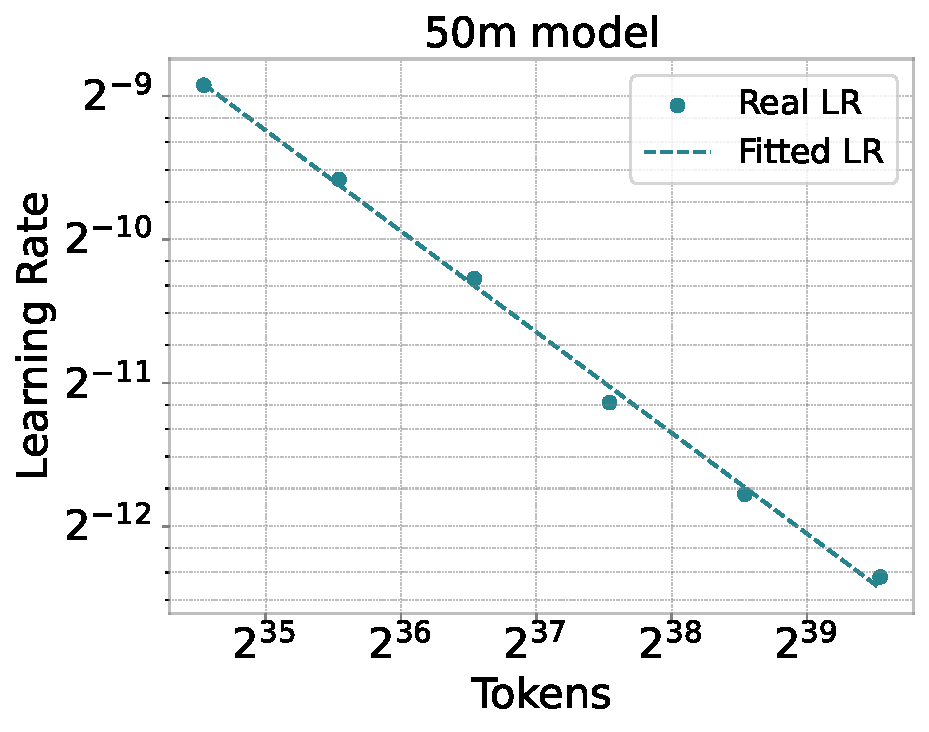
\includegraphics[width=\linewidth]{images/fit_30m.pdf}
    \end{minipage}
    \begin{minipage}[b]{0.45\linewidth}
        \centering
        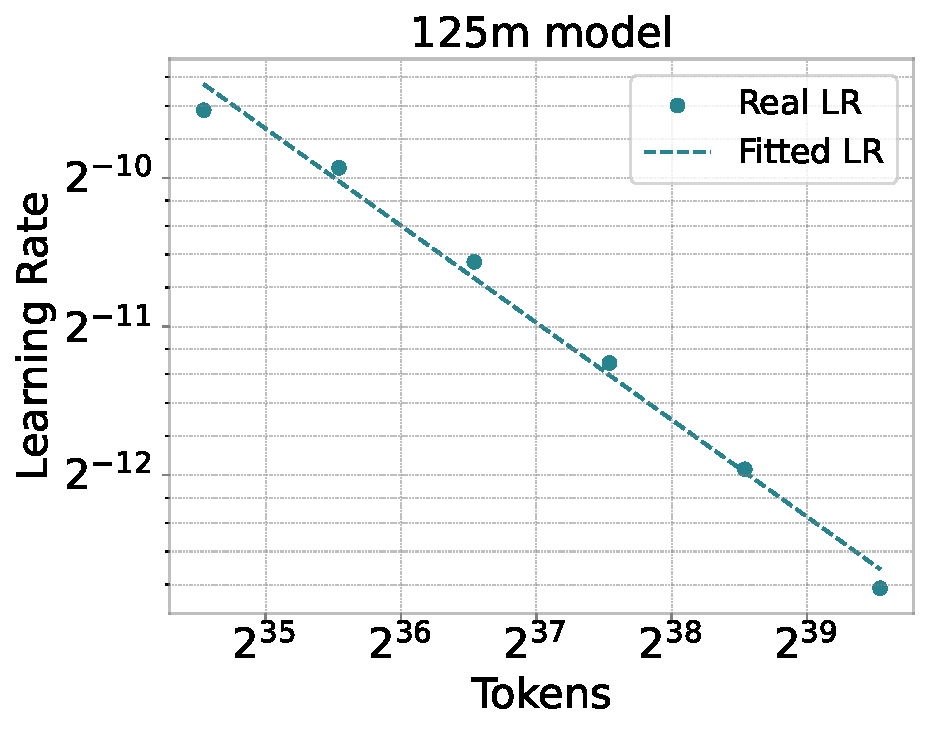
\includegraphics[width=\linewidth]{images/fit_125m.pdf}
    \end{minipage}
    \begin{minipage}[b]{0.45\linewidth}
        \centering
        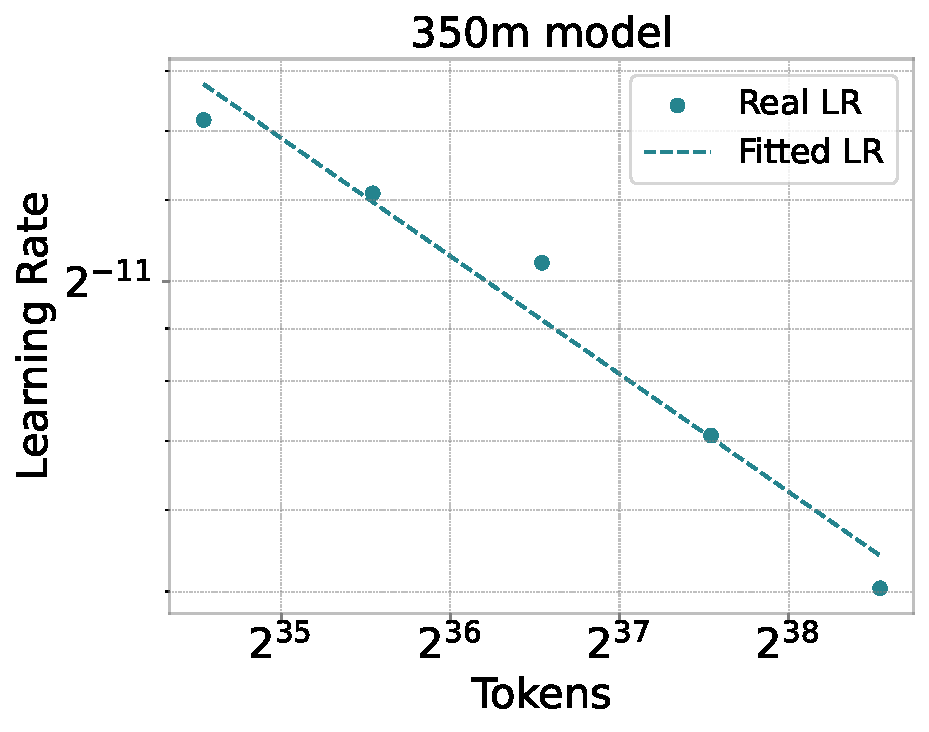
\includegraphics[width=\linewidth]{images/fit_350m.pdf}
    \end{minipage}
    \begin{minipage}[b]{0.45\linewidth}
        \centering
        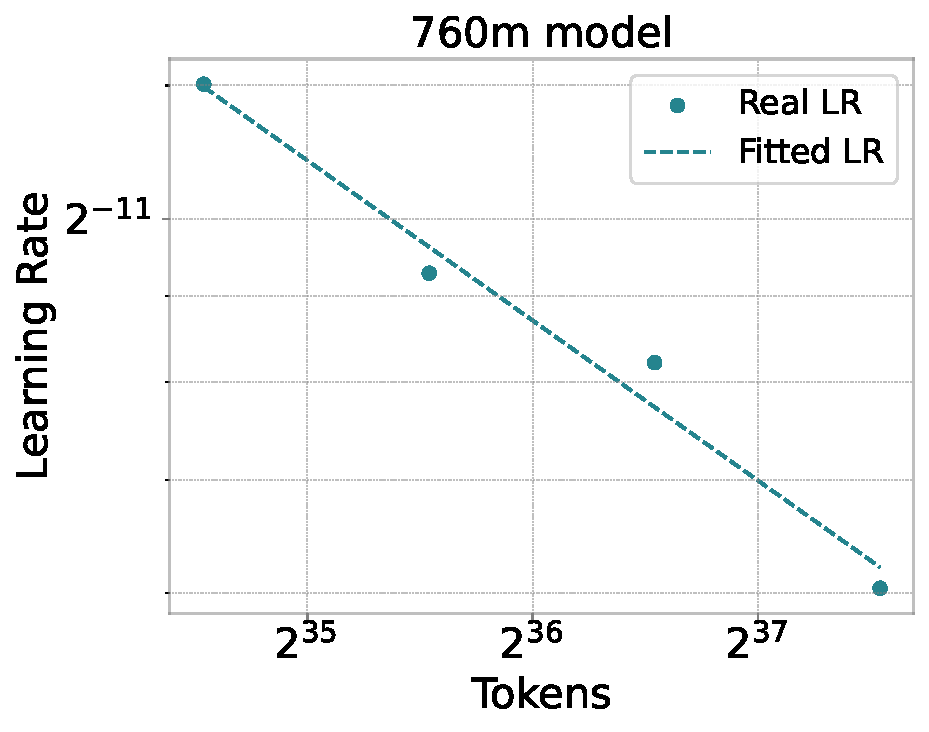
\includegraphics[width=\linewidth]{images/fit_700m.pdf}
    \end{minipage}
    \vspace{-0.3cm}
    \caption{Scaling laws for optimal LR versus token Horizon. We compare the empirically best LR (dots) to the smooth scaling law of \Cref{eq:powerlaw} with fitted constants. The $R^2$ of these fits are in the range 0.99 - 0.96. Across all model sizes, we see that the scaling law provides a good fit to the empirical data. \johan{should be real $LR^*$ instead of LR in legend? Do base 10 if time}}
    \label{fig:4fits}
    \vspace{-0.3cm}
\end{figure}



\subsection{Scaling Laws}

\label{sec:scaling_laws}

We have seen that longer token horizons require smaller LR. We now investigate if this insight allows us to derive scaling laws and do \textit{hyperaprameter-transfer} -- i.e. finding the optimal LR to a long token horizon from experiments on a shorter horizon. To do this we will fit scaling laws to our empirical results. Given some fixed model architecture and training recipe, let ${LR}^*(D)$ denote the optimal LR for some token horizon $D$. We will use the following functional form:
\begin{equation}
\label{eq:powerlaw}
LR^*(D) = B D^{-\beta}
\end{equation}
Here $B$ and $\beta$ are two constants \rebuttal{independent of $D$} that might e.g. depend on the model architecture. Taking the logarithm of both sides of \Cref{eq:powerlaw} we get
\begin{equation}
\label{eq:logpowerlaw}
\log  \big[ LR^*(D) \big] = \log B  - \beta \log D
\end{equation}
We thus have a linear equation in the unknowns $\log B, \beta$, and can fit these to our experimental results with least squares. Specifically, we use the minimizer of the quadratic fits of \Cref{fig:4curves} as the data points $LR^*$. Fitting \Cref{eq:logpowerlaw} gives good fits -- the curves for four models are shown in \Cref{fig:4fits}. The $R^2$ of these fits are in the range 0.99-0.96 (see \Cref{table:r2_scaling} in \Cref{appendix:hps} for exact values), a rather high number. In \Cref{fig:single_fit_1b2b} in the Appendix we also show the fits for the 1.3B and 2.7B models, which also show a good fit. In \Cref{fig:gated_both} in the Appendix we repeat these experiments on a small scale by using the Llama architecture on the smallest 50m model, and find that the $\beta$ transfer well across architectures when using the same model size.  In \Cref{fig:fixed_tokens} we repeat these experiments by doing multiple epochs over a fixed dataset of 25B tokens, and observe similar scaling behavior.

To \textit{evaluate} \rebuttal{the predictive power of} the scaling laws we cannot solely rely on $R^2$ as that is essentially a measure of training loss. We instead need to evaluate the fit on some held-out data. To simulate hyperparameter transfer we thus consider fitting the constants $\log B, \beta$ on token horizons $25B, 50B$ and $100B$ -- and then use these constants to predict the optimal LR at longer horizons. We will use the optimal LR we have empirically found with quadratic fits as the correct LR. The results are illustrated for the 50m model in \Cref{table:simulated_transfer}. We see a reasonably good fit with a relative error of 10-15\% -- a clear improvement over not scaling LR at all which has a relative error of $>250\%$. We thus conclude that \textbf{it is possible to perform hyperparameter transfer across token horizons with our scaling laws}. \Cref{table:simulated_transfer} is repeated for more models with similar fits in \Cref{appendix:experimental_data}.



\begin{table}[t]
    \begin{center}
\setlength{\tabcolsep}{4pt}
\begin{tabular}{lllllll}
\toprule
&    25B &      50B &   100B &      200B &  400B &  800B \\
\midrule
Optimal LR &   \scinot{1.54}{-3} & \scinot{9.79}{-4} & \scinot{6.06}{-4} & \scinot{3.33}{-4} & \scinot{2.14}{-4} & \scinot{1.71}{-4} \\    
Predicted LR &            &               &               & \scinot{3.81}{-4} & \scinot{2.39}{-4} & \scinot{1.50}{-4} \\      
\midrule
Ratio &   &               &             & 0.873 & 0.894 & 1.14 \\\bottomrule
\end{tabular}
    \end{center}
    \caption{Simulated hyperparameter transfer across token horizons for a 50m model. We use the empirically measured optimal LR at 25,50 and 100B tokens to estimate the optimal LR at longer horizons by fitting the constants of \Cref{eq:logpowerlaw}. We find a reasonable fit when scaling up the horizon to 800B tokens, with a relative error of 10-15 \%. The relative error of using the best LR at the 100B horizon for an 800B horizon is $>$ 250\%. \rebuttal{The scaling laws thus have predictive power.}}
    \vspace{-0.3cm}
\label{table:simulated_transfer}
\end{table}
